\documentclass[11pt]{article}
\usepackage[T1]{fontenc}
\usepackage[utf8]{inputenc}
\usepackage{lmodern,amsmath,amssymb,amsthm,mathtools,microtype,enumitem}
\usepackage[a4paper,margin=27mm]{geometry}
\usepackage[hidelinks]{hyperref}
\usepackage{tikz}
\setlength{\emergencystretch}{2em}
\newtheorem{theorem}{Theorem}[section]
\newtheorem{lemma}[theorem]{Lemma}
\newtheorem{corollary}[theorem]{Corollary}
\theoremstyle{remark}\newtheorem{remark}[theorem]{Remark}
\newcommand{\R}{\mathbb R}\newcommand{\Q}{\mathbb Q}\newcommand{\Z}{\mathbb Z}
\newcommand{\CP}{\mathcal{CP}}\newcommand{\COP}{\mathcal{COP}}
\newcommand{\Ry}{\mathcal R}\newcommand{\tr}{\operatorname{tr}}
\newcommand{\diag}{\operatorname{diag}}\newcommand{\cone}{\operatorname{cone}}
\newcommand{\ip}[2]{\langle #1,#2\rangle}\newcommand{\trans}{^{\mathsf T}}
\newcommand{\norm}[1]{\lVert #1\rVert}
\DeclareMathOperator{\dist}{dist}
\newtheorem{proposition}[theorem]{Proposition}
\theoremstyle{definition}\newtheorem{definition}[theorem]{Definition}
\newcommand{\T}{^{\mathsf T}}\newcommand{\Min}{\operatorname{Min}}
\title{Pivot lower bounds and lattice geometry in completely positive matrix separation}
\author{Harman Singh\\[3pt]\normalsize University of Waterloo, Canada\\
\normalsize\href{mailto:h56singh@uwaterloo.ca}{h56singh@uwaterloo.ca}}
\date{}
\hypersetup{pdftitle={Pivot lower bounds and lattice geometry in completely positive matrix separation},pdfauthor={Harman Singh}}
\begin{document}
\maketitle
\begin{abstract}
A symmetric matrix is completely positive if it is a sum of outer products of nonnegative vectors. When such a factorization does not exist, a copositive matrix can certify the failure. A simplex-type search looks for these certificates by moving between neighboring matrices while improving a linear objective. We show that this search can require exponentially many steps even when a short separator exists. Under explicit, finitely checkable conditions on a single nonmember, we construct positive-definite, entrywise-positive inputs for which every strictly improving adjacent-pivot choice is slow relative to the input bit length. The bound survives perturbations and applies to all starts in a fixed bounded region of the relevant face. It also survives diagonal corrections to combinations of previous pivot directions. Independently, we show that certain convex sets defined by integer quadratic inequalities have only finitely many local adjacency patterns and graph balls whose size grows polynomially with distance. Graphical constructions supply distinct qualifying seeds, including nonmembers whose every proper principal submatrix is completely positive.
\end{abstract}
\noindent\textbf{Keywords:} completely positive matrix; copositive matrix; adjacent pivot; lattice epigraph; graph growth.\\
\textbf{2020 Mathematics Subject Classification:} 15B48; 90C49; 11H55.
\section{Introduction}\label{sec:intro}
A real symmetric matrix can have nonnegative entries and nonnegative eigenvalues without being a sum of rank-one matrices made from nonnegative vectors. A matrix that does admit such a sum is called \emph{completely positive}. In symbols,
\[
 A=\sum_{j=1}^k u_ju_j\T,\qquad u_j\ge0.
\]
In matrix orders up to four, nonnegative entries and positive semidefiniteness are enough. From order five onward, they are not \cite{Diananda,MM}. Completely positive matrices therefore pose a natural question in matrix factorization: how can we prove that an apparently well-behaved matrix has no such representation?

There is a direct form of evidence for nonmembership. A symmetric matrix $W$ is \emph{copositive} when $x\T Wx$ is nonnegative for every nonnegative vector $x$. If $W$ is copositive but $\tr(AW)$ is negative, then $A$ cannot be completely positive: every allowed rank-one term would have nonnegative pairing with $W$. The entries of such a $W$ may be short to describe, even when finding it is difficult. A short certificate of nonmembership and a short search for that certificate are different things.

One way to look for $W$ is to follow neighboring vertices of a convex set of copositive matrices. The simplex-type method of Dutour Sikiri\'c, Sch\"urmann and Vallentin \cite{DSV} uses vertices determined by integer vectors at which a quadratic form attains its prescribed minimum. These vertices are known as \emph{perfect copositive matrices}. At each step, a pivot follows an edge to a neighboring vertex that lowers the objective $\tr(AP)$. The method may also discover a separating matrix without completing another pivot. Its appeal is that it works with local information: the current vertex, its neighboring directions, and prescribed certificate tests.

This leaves a question that a long example path does not answer. Can a choice of a different improving neighbor avoid a bad route? Could a test applied to the current direction find a certificate before the route becomes long? A lower bound for one prescribed sequence settles neither question. We study the stronger requirement that \emph{every strictly improving adjacent choice} is forced to continue and that the permitted local certificate tests fail along the entire initial part of the search.

Our first result gives a general way to construct such inputs. Begin with a rational matrix $B$ that is positive definite, has strictly positive entries, and is not completely positive. Require an explicit copositive separator and a positive description of one principal block in terms of the minimizing vectors of a suitable perfect matrix. These conditions are finite and can be certified exactly. They do not purport to characterize all nonmembers. They identify a class of starting examples, which we call \emph{certified seeds}, from which difficult local-search instances can be generated systematically.

Fix one such seed and a bounded region of initial vertices in the corresponding fixed-block face. For any integer $m\ge1$, a diagonal scaling with parameter $N$ proportional to $m+1$ produces an input requiring at least $m$ pivots for \emph{every} permitted improving choice from \emph{every} such initial vertex. The constants depend on the fixed seed and starting region. The entries of the input need only a number of binary digits proportional to $\log(m+1)$. An explicitly constructed rational copositive separator has a description of comparable length. The result remains true in a specified ball around the input. These matrices are positive definite and strictly entrywise positive, so the two elementary tests do not detect nonmembership. Thus the gap is not between the existence of a certificate and its size: it is between the existence of a short certificate and the number of local moves needed to encounter one.

The mechanism comes from a second, geometric result. Fix a positive-definite principal block $H$, and let the last column and diagonal entry of a symmetric matrix vary. Requiring its quadratic form to be at least one on nonnegative integer vectors with positive last coordinate defines a convex region. We call it a \emph{fixed-block lattice epigraph}. Its vertices are joined by edges, giving a graph in which distance counts adjacent moves. We prove, for every real positive-definite $H$, that integer changes of coordinates reduce the possible local configurations to finitely many types. In particular, the graph has bounded degree, and the number of vertices reachable within $R$ edge moves grows on the order of $R^r$ when $H$ has order $r$. This geometric statement needs neither a completely positive nonmember nor a chosen objective function. A related full-lattice version has the large-scale geometry of the integer lattice. The distances here are measured \emph{inside the fixed-block region}, which is a face when $H$ is perfect; the result makes no assertion about shortcuts outside it.

The hard inputs are not confined to the familiar five-cycle example. We give distinct graphical seed classes, as well as examples built from different perfect principal blocks. One construction produces a positive-definite, entrywise-positive nonmember of order thirteen for which \emph{every proper principal submatrix is completely positive}. Hence even checking every smaller principal submatrix exactly would not find the obstruction. We also consider stronger local tests that add diagonal matrices to combinations of previously used pivot directions. For our inputs these tests cannot separate during the forced prefix. The decomposition fact used for the resulting arrow-shaped matrices is classical \cite{SPN}; the consequence for all stored directions is part of our lower-bound result.

The simplex-type search and perfect copositive matrices were developed in earlier work \cite{DSV}; the geometry of their neighbors and related perfect-form constructions have also been studied \cite{DS,OS}. Inhomogeneous reduction proves finiteness of perfect quadratic functions up to affine integer changes of variables and scaling \cite[Section~5]{Inhom}. Here we keep a prescribed positive-definite block, include every positive last integer coordinate and the boundary imposed by nonnegativity, and prove exact intrinsic graph growth. The present amplification also adds an all-choice, finite-bit-length lower bound from a certified class of seeds. Our theorem does \emph{not} rule out algorithms that construct unrelated separators, jump between nonadjacent vertices, or choose distant starting points depending on the input. Nor does it settle eventual termination of a suitable pivot rule, as asked in \cite[Conjecture~3.2]{DSV}. The proof first establishes the fixed-block geometry, then uses the seed conditions to prevent every improving extreme direction from leaving that face too early. Concrete graphical seeds and stronger-test barriers complete the argument.

\section{Certificates, pivots, and main results}\label{sec:model}
The search compares the input with one vertex at a time. It may stop with a separating certificate or move along an improving edge. We first specify those choices; the geometry theorem below concerns the underlying set independently of any search.

\subsection{The local model}
Let $\mathbb S^n$ denote the real symmetric matrices, with pairing $\ip A P=\tr(AP)$ and Frobenius norm $\norm P_F^2=\tr(P^2)$. We write $P[v]=v\T Pv$. The notation $A\succeq0$ means positive semidefiniteness, whereas $A\ge0$ means that every entry is nonnegative. A matrix with both properties is called \emph{doubly nonnegative}. The closed dual cones of interest are
\[
 \CP_n=\cone\{uu\T:u\in\R_+^n\},\qquad
 \COP_n=\{P:P[x]\ge0\text{ for every }x\ge0\}.
\]
The duality follows by testing the rank-one generators. Closedness of $\CP_n$ follows, for example, by intersecting with the trace-one hyperplane: this base is the convex hull of the compact set $\{uu\T:u\ge0,\norm u_2=1\}$.

The normalized integer constraints define the copositive Ryshkov set
\begin{equation}\label{eq:ryshkov}
 \Ry_n=\{P\in\mathbb S^n:P[v]\ge1\text{ for every }0\ne v\in\Z_+^n\}.
\end{equation}
An integer vector with $P[v]=1$ is \emph{active}, or minimizing. If its active matrices $vv\T$ span $\mathbb S^n$, then $P$ is a vertex, also called a normalized perfect copositive matrix. The vertices used here are strictly copositive, meaning $P[x]>0$ for every nonzero $x\ge0$. This ensures that finitely many constraints describe a neighborhood, as proved in Section~\ref{sec:face}. Their tangent cones are therefore the polyhedral cones
\begin{equation}\label{eq:tangent}
 \mathcal T(P)=\{R:R[v]\ge0\text{ for every active }v\}.
\end{equation}
An extreme ray is a one-dimensional face of this cone. It is \emph{improving} for $A$ when $\ip A R<0$. Following it either reaches a neighboring vertex along a bounded edge or continues in a recession direction. A move along a bounded edge is one \emph{adjacent pivot}. A rational ray has a \emph{primitive integral generator}: clear the entry denominators and divide by their greatest common divisor.

At a departure vertex the rule may test the current $P$, the selected improving ray $R$, or
\begin{equation}\label{eq:storedtest}
 Q=\sum_{j=0}^k\beta_jR_j+\Lambda,
 \qquad \beta_j\in\R,\quad\Lambda\text{ real diagonal},
\end{equation}
where the $R_j$ are previously stored improving directions and the currently selected direction. A test succeeds only when its candidate is copositive and has negative pairing with $A$. This includes $R+\tau I$ for every real $\tau$, and arbitrary diagonal corrections of a single ray. If no test succeeds, the rule makes the adjacent pivot. Choosing among improving extreme rays may use the full input and history, or randomization; no computational restriction is imposed on that choice.

The current-vertex and ray tests are the nonmembership exits of Procedure~3 in \cite{DSV}. The tests \eqref{eq:storedtest} enlarge that local model. A separate construction of an unrelated certificate, a nonadjacent move, or an initial vertex outside the prescribed region is outside it. No claim about the cost of recognizing an arbitrary copositive matrix is implicit in this definition.

\subsection{Amplification from a finite seed}
Informally, a seed is a small nonmember with a known separator and a principal block that favors one perfect matrix strictly. The strict preference has a finite certificate: a positive combination of its active rank-one matrices. It will make leaving the corresponding face expensive after scaling.

\begin{definition}[Certified seed]\label{def:seed}
Let $n=r+1$. A certified seed consists of the following rational data:
\begin{enumerate}[label=(\roman*),itemsep=2pt]
\item a positive definite perfect vertex $H\in\Ry_r$;
\item a positive definite matrix $B=\begin{pmatrix}C&c\\c\T&a\end{pmatrix}$, every entry of which is strictly positive;
\item vectors $v_j\in\Z_+^r$ with $H[v_j]=1$, whose matrices $v_jv_j\T$ span $\mathbb S^r$, and positive coefficients $\lambda_j\in\Q$ satisfying
\begin{equation}\label{eq:reserve}
 C=\sum_j\lambda_jv_jv_j\T;
\end{equation}
\item a rational $W\in\COP_n$ with $\ip W B=-\gamma<0$, together with a proof of its copositivity.
\end{enumerate}
\end{definition}

These are sufficient conditions, not a characterization of all nonmembers. For rational $H\succ0$, the integer constraints below one can be checked in a finite ball, using $\lambda_{\min}(H)\ge1/\tr(H^{-1})$. The spanning and reserve conditions are exact rational linear algebra. Copositivity still requires the supplied proof or an exact finite decision method. Finite certification here does not mean polynomial-time verification as the order varies.

The following theorem turns every such seed into an input family. The scale grows linearly with the requested number of pivots, while the number of binary digits grows logarithmically. All initial vertices in the stated bounded region are covered at once.

\begin{theorem}[Certified-seed amplification]\label{thm:amplification}
Fix a certified seed, a number $b_0\ge0$, and the positive rational constants $s_0,\theta,\zeta$ and integer $\Gamma$ in \eqref{eq:robustconstants}--\eqref{eq:Gamma}. For $m\ge1$, set
\begin{equation}\label{eq:amplified}
 N=\Gamma(m+1),\quad D_N=\diag(NI_r,1),\quad
 A_N=\frac{D_NBD_N}{s_0N^2},\quad
 W_N=D_N^{-1}WD_N^{-1}+\frac\theta{N^2}I_n.
\end{equation}
Every symmetric $A$ satisfying
\begin{equation}\label{eq:ball}
 \norm{A-A_N}_F\le\frac\zeta{s_0N^2}
\end{equation}
has the following properties.
\begin{enumerate}[label=(\alph*),itemsep=3pt]
\item $\norm A_F\le1$, $A\succ0$, every entry is positive, and $A\notin\CP_n$.
\item From every vertex of $\Ry_n$ with leading block $H$ and cross column of norm at most $b_0$ in $\norm\cdot_\infty$, every local rule above makes at least $m$ adjacent pivots. At every departure vertex before the $m$th pivot, an improving extreme ray exists, every such ray reaches a finite neighbor in the same fixed-block face, and none of the permitted certificates separates.
\item The same rational $W_N$ separates the entire ball, with
\begin{gather}\label{eq:ampmargin}
 W_N[x]\ge\frac\theta{N^2}\norm x_2^2\quad(x\ge0),\qquad
 \norm{W_N}_F\le w+n\theta,\\
 \label{eq:ampdistance}
 \ip{W_N}A\le-\frac\gamma{2s_0N^2},\qquad
 \dist_F(A,\CP_n)\ge\frac\gamma{2s_0(w+n\theta)N^2},
\end{gather}
where $w=1+\sum_{ij}|W_{ij}|$.
\end{enumerate}
For this fixed seed and starting region, the binary lengths of the rational centers and separators are $O(\log(m+1))$. The center's input length, also when augmented by the logarithm of reciprocal distance to $\CP_n$, is $\Theta(\log(m+1))$. The forced prefix is therefore exponential in either measure. Every visited vertex and primitive integral extreme-ray generator in the prefix has $O(\log(m+1))$ bit height.
\end{theorem}

The initial vertex can be chosen using the input within this fixed region. The theorem does not allow the region to grow with $m$. Nor is the bit-length conclusion asserted for arbitrary rational points of the ball, which can have arbitrarily long encodings.

The stronger correction clause has a useful exact formulation. Its force comes from the shape of the stored directions, rather than from bounds on the test coefficients.

\begin{corollary}[Stored-direction correction barrier]\label{cor:stored}
At any covered prefix vertex, let $R_1,\ldots,R_k$ be any stored improving rays from covered departure vertices. For arbitrary real $\beta_j$ and arbitrary real diagonal $\Lambda$, if $Q=\sum_j\beta_jR_j+\Lambda$ is copositive, then $\ip A Q\ge0$. The same holds for any combination also including a currently tested improving extreme ray.
\end{corollary}

\subsection{The independent fixed-block geometry}
For arbitrary real $H\succ0$ of order $r$, the inequalities involving a positive last integer coordinate define
\begin{equation}\label{eq:epigraph}
 \mathcal E_H=\{(b,c):c\ge g_H(b)\},\qquad
 g_H(b)=\sup_{\substack{u\in\Z_+^r\\y\in\Z_{\ge1}}}
 \frac{1-u\T Hu-2yb\T u}{y^2}.
\end{equation}
Its bounded-edge graph has the vertices of $\mathcal E_H$ as nodes and bounded edges as graph edges. When $H$ is a perfect vertex of $\Ry_r$, this is the graph inside the face with leading block $H$. For a general $H$, \eqref{eq:epigraph} is studied on its own; the zero-last-coordinate inequalities need not hold.

An integer shear replaces the first $r$ coordinates $u$ by $u-ay$ for an integral vector $a$. The next result says that this removes the unbounded location of a vertex from its local description.

\begin{theorem}[Finite local configurations]\label{thm:finite}
Let $H\succ0$ be real of order $r\ge1$. There are constants $Y_H,K_H$ such that every active pair has $1\le y\le Y_H$, and at each vertex an integral shear puts every active numerator in $[-K_H,K_H]^r$. The sheared vertices and their local adjacency configurations in this graph belong to finite containing lists depending only on $H$.

If $H$ is rational, one common integer denominator works for the coordinates of every vertex of $\mathcal E_H$. If in addition $H$ is a perfect vertex, all primitive integral extreme rays of the full Ryshkov tangent cones have uniformly bounded entries after the same shear. Explicit bounds are given in Proposition~\ref{prop:templates} and Lemma~\ref{lem:shearedrays}.
\end{theorem}

The containing lists may include configurations that never occur. No algorithm deciding realization at an arbitrary integral translate is asserted. In particular, the full Ryshkov ray conclusion uses more than a bound on rays within the face.

The graph consequence holds without a seed or an objective. Here and below, graph distance counts edges within this fixed-block set.

\begin{theorem}[Intrinsic graph growth]\label{thm:growth}
For every real $H\succ0$ of order $r\ge1$, the bounded-edge graph of $\mathcal E_H$ is connected and has bounded degree. For each vertex $v$, there are constants $c_v,C_v>0$ such that, for all sufficiently large integers $R$,
\begin{equation}\label{eq:growth}
 c_vR^r\le |B_{\mathrm{graph}}(v,R)|\le C_v(1+R)^r.
\end{equation}
For the full-lattice epigraph $\mathcal E_H^{\Z}$, defined by allowing $u\in\Z^r$ in \eqref{eq:epigraph}, the graph is quasi-isometric to $\Z^r$. The two epigraphs coincide locally wherever
\begin{equation}\label{eq:deep}
 z=-H^{-1}b,\qquad z_i>\sqrt{(H^{-1})_{ii}}\quad(1\le i\le r).
\end{equation}
\end{theorem}

Quasi-isometry means that graph and lattice distances differ by at most fixed multiplicative and additive constants, with every graph vertex a bounded distance from the chosen lattice-indexed vertices. Integral shears are automorphisms of the full-lattice graph. They need not preserve the orthant epigraph. Neither theorem compares intrinsic distance with a path allowed to leave the face.

\subsection{An explicit canonical family}
Let $T_j$ be the tridiagonal matrix with diagonal $1$, adjacent off-diagonal entries $-1/2$, and other entries zero. Section~\ref{sec:canonicalseed} gives a five-cycle seed with leading block $T_{n-1}$. It yields the following fully explicit specialization, including numerical robustness and separator bounds. The constants defining $A_{n,t},W_{n,t}$ and $N$ appear in Appendix~\ref{app:canonical}.

\begin{corollary}[Canonical start and five-cycle seed]\label{cor:canonical}
For every $n\ge5$ and integer $t\ge1$, there are explicit rational $A_{n,t}$ and $W_{n,t}$ such that every $A$ with
\[
 \norm{A-A_{n,t}}_F\le\frac1{1600n^4N^2}
\]
is positive definite, strictly entrywise positive, outside $\CP_n$, and has $\norm A_F\le1$. Every permitted improving adjacent rule from $T_n$ makes at least $t$ pivots. No vertex, selected ray, scalar identity correction, or corrected stored-ray combination separates during this prefix. One separator works throughout the ball and satisfies
\begin{gather}\label{eq:canonicalmargins}
 W_{n,t}[x]\ge\frac{\norm x_2^2}{20nN^2}\quad(x\ge0),\qquad
 \norm{W_{n,t}}_F\le6,\\
 \ip A{W_{n,t}}\le-\frac1{6nN^2},\qquad
 \dist_F(A,\CP_n)\ge\frac1{36nN^2}.
\end{gather}
For fixed $n$, input and separator lengths are $O_n(\log(t+1))$, and the pivot count is exponential in the input length, also with the reciprocal-distance term included.
\end{corollary}

\section{Geometry of fixed-block lattice epigraphs}\label{sec:movement}
An adjacent edge preserves some integer quadratic constraint at both endpoints. This shared constraint controls movement even when the edge is far from the origin. For $H=(1)$, for example, the matrices with $(b,c)=(-1/2,1)$ and $(-3/2,3)$ are adjacent: they preserve the active vectors $(1,0)$ and $(1,1)$, and the second endpoint gains $(2,1)$. Both forms are integer changes of $u^2-uy+y^2$, whose integer minimum is one; their shared equalities define a line, and the remaining inequalities stop it at these endpoints. Figure~\ref{fig:edge} shows the edge in \eqref{eq:epigraph}.

\begin{figure}[htbp]
\centering
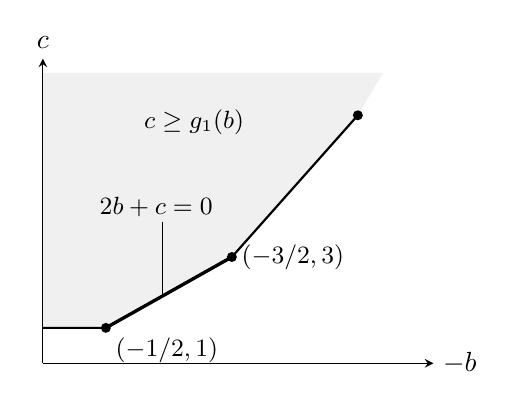
\begin{tikzpicture}[x=1.6cm,y=0.45cm,>=stealth]
\fill[gray!12] (0,1)--(0.5,1)--(1.5,3)--(2.5,7)--(2.7,8.2)--(0,8.2)--cycle;
\draw[->] (0,0)--(3.1,0) node[right] {$-b$};
\draw[->] (0,0)--(0,8.6) node[above] {$c$};
\draw[thick] (0,1)--(0.5,1)--(1.5,3)--(2.5,7);
\draw[very thick] (0.5,1)--(1.5,3);
\fill (0.5,1) circle (1.8pt) node[below right] {\small $(-1/2,1)$};
\fill (1.5,3) circle (1.8pt) node[right] {\small $(-3/2,3)$};
\fill (2.5,7) circle (1.8pt);
\node at (1.2,6.8) {\small $c\ge g_1(b)$};
\node at (0.9,4.4) {\small $2b+c=0$};
\draw[thin] (0.95,4.0)--(0.95,1.9);
\end{tikzpicture}
\caption{An explanatory slice with $H=(1)$, not a hard input from Theorem~\ref{thm:amplification}. Labels give $(b,c)$; the horizontal axis is $-b$. The highlighted edge preserves the constraint $2b+c=0$.}
\label{fig:edge}
\end{figure}

For general $H\succ0$, the defining inequalities are
$H[u]+2yb\T u+cy^2\ge1$ for $u\in\Z_+^r$ and $y\ge1$ integral. The epigraph \eqref{eq:epigraph} is their intersection. The first bound concerns the cross column $b$, not every entry of the block matrix.

\begin{theorem}[Movement along a bounded edge]\label{thm:movement}
If $(b,c)$ and $(b',c')$ are the endpoints of a bounded edge of $\mathcal E_H$, then
\begin{equation}\label{eq:movement}
 |b_i'-b_i|\le\frac12+2\sqrt{H_{ii}}\qquad(1\le i\le r).
\end{equation}
For $H=T_r$, this gives $\norm{b'-b}_\infty\le5/2$, independently of the location and order.
\end{theorem}

We compare each endpoint with a continuous quadratic minimum. The comparison first bounds the last coordinate of every active integer vector, then leaves a common term that cancels across an edge.
\subsection{Comparison with the continuous minimum}
Let $z=z(b)$ be the unique minimizer of
$x\trans Hx+2b\trans x$ over $x\ge0$, and put $\ell=b+Hz$.
Positive definiteness gives existence and uniqueness. The optimality conditions are
\begin{equation}\label{eq:kkt}
 z\ge0,\qquad \ell\ge0,\qquad z_i\ell_i=0\quad(1\le i\le r).
\end{equation}
Thus the continuous minimum is $-z\trans Hz$. We choose a fixed approximation scale to compare the discrete constraints uniformly with this minimum. The constants below will measure a positive gap and bound the last coordinate of active integer vectors. Choose an integer $q\ge2$ such that $\norm H_2r/q^2\le1/2$, where $\norm H_2$ is the spectral norm, and set
\begin{equation}\label{eq:gapconstants}
 \kappa=\frac1{2q^{2r}},\qquad Y=2q^r.
\end{equation}

\begin{lemma}[A positive gap and bounded active vectors]\label{lem:gap}
For every $b\in\R^r$,
\begin{equation}\label{eq:gap}
 z\trans Hz+\kappa\le g_H(b)\le z\trans Hz+1.
\end{equation}
The supremum in \eqref{eq:epigraph} is attained. Every active pair $(u,y)$ at $(b,g_H(b))$ satisfies, with $e=u-yz$,
\begin{equation}\label{eq:active}
 y\le Y,\qquad
 e\trans He+2y\ell\trans u
   =1-y^2\bigl(g_H(b)-z\trans Hz\bigr)\le1.
\end{equation}
The epigraph is locally polyhedral. At every vertex, $0\le\ell_i\le1/2$ for each $i$.
\end{lemma}
\begin{proof}
The comparison is based on the identity
\begin{equation}\label{eq:complete}
 \frac{1-u\trans Hu-2yb\trans u}{y^2}
 =z\trans Hz+\frac{1-e\trans He-2y\ell\trans u}{y^2}.
\end{equation}
To obtain it, substitute $b=\ell-Hz$ and use $\ell\trans z=0$. Both terms subtracted from $1$ on the right are nonnegative. Since $y\ge1$, this proves the upper bound in \eqref{eq:gap}.

For the lower bound we need one integer pair close to the continuous minimizer after scaling. Let $S=\{i:z_i>0\}$ and $s=|S|$, and let $z_S$ be the restriction of $z$ to $S$. If $s=0$, the pair $u=0,y=1$ gives the assertion. Otherwise place the $q^s+1$ coordinatewise fractional-part vectors
\[
 \{kz_S\},\qquad 0\le k\le q^s,
\]
in $q^s$ half-open boxes of side $1/q$. Two lie in the same box. Subtracting them gives $1\le y\le q^s\le q^r$ and integers $u_i$ such that $|u_i-yz_i|\le1/q$ on $S$. Put $u_i=0$ outside $S$. These integers are nonnegative: a negative integer would have distance at least one from the nonnegative number $yz_i$. Complementarity gives $\ell\trans u=0$, and
\[
 (u-yz)\trans H(u-yz)\le\norm H_2\frac r{q^2}\le\frac12.
\]
The last fraction in \eqref{eq:complete} is therefore at least $1/(2q^{2r})$. This proves the lower bound using the elementary simultaneous approximation argument, without any restriction on rationality of $b$ or $z$.

If $y>Y$, the right side of \eqref{eq:complete} is at most
$z\trans Hz+1/y^2<z\trans Hz+\kappa$.
For the finitely many remaining $y$, any value at least $z\trans Hz+\kappa$ requires $(u-yz)\trans H(u-yz)\le1$. A bounded ellipsoid contains only finitely many integer vectors. Thus the supremum is attained; multiplying \eqref{eq:complete} by $y^2$ proves \eqref{eq:active}.

These are local finiteness bounds as well. The minimizer $z(b)$ is continuous; this follows from the variational inequalities and strong convexity, which give
$\norm{z(b)-z(b')}_2\le\norm{b-b'}_2/\lambda_{\min}(H)$.
On a small neighborhood, $z$ stays bounded. All constraints that can attain the supremum there have $y\le Y$ and $(u-yz)\trans H(u-yz)\le1$, hence come from one finite list. This proves local polyhedrality.

Finally, a vertex must lie on the graph of $g_H$. Its active affine normals $(2u/y,1)$ span $\R^{r+1}$. For each $i$ at least one active $u$ has $u_i\ge1$, since otherwise their $i$th components would all vanish. Equation~\eqref{eq:active} then gives
$2y\ell_i u_i\le1$, and hence $\ell_i\le1/2$.
\end{proof}

\begin{proof}[Proof of Theorem~\ref{thm:movement}]
The epigraph is full dimensional and locally polyhedral. A bounded edge has a common active constraint $(u,y)$ at its endpoints: the equalities defining its relative interior remain equalities at both ends. At the first endpoint,
\begin{equation}\label{eq:shared}
 b+H(u/y)=\ell+He/y.
\end{equation}
Cauchy--Schwarz for the inner product defined by $H$ gives
\[
 |(He)_i|^2\le H_{ii}\,e\trans He\le H_{ii}.
\]
Together with $0\le\ell_i\le1/2$, this puts the $i$th coordinate of \eqref{eq:shared} in the interval
\[
 \left[-\frac{\sqrt{H_{ii}}}{y},\,
       \frac12+\frac{\sqrt{H_{ii}}}{y}\right].
\]
The second endpoint has the same $u$ and $y$, so subtracting cancels the term $H(u/y)$. The interval length is at most $1/2+2\sqrt{H_{ii}}$, proving \eqref{eq:movement}. Neither simplicity of a vertex nor $y=1$ has been assumed.
\end{proof}



\subsection{Integer shears and finite configurations}
The active vectors can grow with the location of a vertex. Subtracting the integer part of the continuous minimizer removes that growth. Choose an integer $t_H\ge1$ with
\begin{equation}\label{eq:alphabet}
 t_H\ge\max_i\sqrt{(H^{-1})_{ii}},\qquad K=Y+t_H,
 \qquad
 \mathcal D_H=\{(v,y)\in\Z^r\times\Z:|v_i|\le K,\ 1\le y\le Y\}.
\end{equation}
For $a\in\Z^r$, write
\begin{equation}\label{eq:shear}
 S_a=\begin{pmatrix}I_r&a\\0&1\end{pmatrix},\quad
 S_a\T\begin{pmatrix}H&b\\b\T&c\end{pmatrix}S_a
 =\begin{pmatrix}H&\bar b\\\bar b\T&\bar c\end{pmatrix},
\end{equation}
so $\bar b=b+Ha$ and $\bar c=c+2b\T a+a\T Ha$. These are changes of integer coordinates. They do not in general preserve the nonnegative orthant.

The next proposition gives the finite containing list used in Theorem~\ref{thm:finite}. Rationality enters only in its denominator conclusion.

\begin{proposition}[Normalized vertices]\label{prop:templates}
At a vertex of $\mathcal E_H$, take $a=\lfloor z\rfloor\in\Z_+^r$. Every active pair $(u,y)$ then has $(u-ay,y)\in\mathcal D_H$. The normalized vertex satisfies
\begin{equation}\label{eq:normalizedbounds}
 |\bar b_i|\le\frac12+\sum_j|H_{ij}|,
 \qquad \kappa\le\bar c\le1+r\norm H_2,
\end{equation}
and is determined by $r+1$ independent equations chosen from
\begin{equation}\label{eq:normalizedequations}
 2yv\T\bar b+y^2\bar c=1-v\T Hv,
 \qquad(v,y)\in\mathcal D_H.
\end{equation}
If $D_HH$ is integral for an integer $D_H\ge1$, every vertex coordinate has denominator dividing
\begin{equation}\label{eq:denominator}
 \Delta_H=D_H\operatorname{lcm}(1,\ldots,F_H),
 \qquad F_H=(r+1)!(2K^2)^{r+1}.
\end{equation}
\end{proposition}
\begin{proof}
Set $f=z-a\in[0,1)^r$. The residual identity \eqref{eq:active} gives
$|u_i-yz_i|\le\sqrt{(H^{-1})_{ii}}\le t_H$, so
$|u_i-a_i y|\le t_H+Y=K$.
Stationarity gives $\bar b=\ell-Hf$. Also $\ell\T a=0$: if $\ell_i>0$, complementarity forces $z_i=a_i=0$. Substituting $b=\ell-Hz$ into the last coordinate of \eqref{eq:shear} therefore gives the cancellation
\begin{equation}\label{eq:shearcancel}
 \bar c=(c-z\T Hz)+f\T Hf.
\end{equation}
The gap lemma and $\norm f_2^2\le r$ prove \eqref{eq:normalizedbounds}.

The invertible coordinate change preserves independence of active affine equations. A vertex has $r+1$ independent ones, and they become \eqref{eq:normalizedequations}. There are finitely many subsets to choose from, giving the finite containing list.

The coefficient matrix in these equations is integral with entries of absolute value at most $2K^2$. Its nonzero determinant has absolute value at most $F_H$, by expansion of the determinant. The right sides have denominators dividing $D_H$. Cramer's rule gives denominators dividing $D_H|\det M|$, hence \eqref{eq:denominator}. Undoing the shear introduces only integer coefficients and entries of $H$, whose denominators already divide $\Delta_H$.
\end{proof}

The same argument controls adjacency patterns. For neighboring vertices let $a=\lfloor z\rfloor$ and $a'=\lfloor z'\rfloor$. Since $z=H^{-1}(\ell-b)$ and $0\le\ell_i\le1/2$,
\[
 \norm{a'-a}_\infty\le
 \norm{H^{-1}}_\infty
 \left(\frac12+\max_i\left(\frac12+2\sqrt{H_{ii}}\right)\right)+1.
\]
Here the matrix infinity norm is the maximum absolute row sum. There are only finitely many relative shifts and normalized endpoint choices. Thus the possible normalized neighbor configurations form a finite containing list as well. The construction uses finite subsets of \eqref{eq:normalizedequations}; it does not decide which candidates are realized.

\subsection{Fixed-block faces and full tangent rays}\label{sec:face}
For amplification, the bound must also control directions that might leave the face. Assume now that $H\succ0$ is a perfect vertex of $\Ry_r$. Keeping its active equalities on vectors $(v,0)$ fixes the leading block, since their squares span $\mathbb S^r$. The resulting face is
\begin{equation}\label{eq:face}
 \mathcal F_H=\left\{P(b,c)=\begin{pmatrix}H&b\\b\T&c\end{pmatrix}:
                 (b,c)\in\mathcal E_H\right\}.
\end{equation}
The inequalities with last coordinate zero already hold because $H\in\Ry_r$.

Every point of $\mathcal F_H$ is strictly copositive. Put $\alpha=c-z\T Hz\ge\kappa$. For $(x,y)\ge0$, completing the square gives
\begin{equation}\label{eq:strictface}
 P(b,c)[(x,y)]=(x-yz)\T H(x-yz)+2y\ell\T x+\alpha y^2.
\end{equation}
If $y>0$, the last term is positive; if $y=0$ and $x\ne0$, the first is positive. On the compact nonnegative unit sphere this gives a positive minimum. A neighborhood of $P$ therefore has a uniform positive copositivity margin. All sufficiently long integer vectors satisfy their inequalities with a strict reserve there, so only finitely many constraints of the \emph{full} $\Ry_n$ are locally relevant. In particular a face vertex is a full-set vertex: its active equations fix the leading block and then all $r+1$ remaining variables.

Finite active vectors now bound primitive integral generators of every full tangent ray, including an escaping direction. Let $n=r+1$ and $d=n(n+1)/2$.

\begin{lemma}[Uniform sheared ray bound]\label{lem:shearedrays}
At a vertex of $\mathcal F_H$, with $a=\lfloor z\rfloor$, every primitive integral extreme tangent ray $R$ of the full $\Ry_n$ satisfies
\begin{equation}\label{eq:shearedrays}
 |(S_a\T RS_a)_{ij}|\le E_*,
 \qquad E_*=(d-1)!(2K^2)^{d-1}.
\end{equation}
Writing $R=\begin{pmatrix}D&w\\w\T&s\end{pmatrix}$ and $T=1+\norm a_1$, one has
\begin{equation}\label{eq:rayblocks}
 |D_{ij}|\le E_*,\qquad |w_i|\le E_*T,\qquad |s|\le E_*T^2.
\end{equation}
\end{lemma}
\begin{proof}
An active vector $(u,0)$ has $H[u]=1$, hence $|u_i|\le t_H$, and is unchanged by the shear. Every other active vector belongs to $\mathcal D_H$ in sheared coordinates. In upper-triangular matrix coordinates, the integer normal of an active equation has coefficients $v_i^2$ and $2v_iv_j$, of absolute value at most $2K^2$.

The full tangent cone is pointed and full dimensional. An extreme ray annihilates $d-1$ independent active equations. For their $(d-1)\times d$ coefficient matrix, the signed maximal minors form a nonzero vector in the one-dimensional nullspace. Each minor is at most $E_*$ in absolute value. Choosing its sign and dividing by the greatest common divisor gives the primitive generator and cannot increase that bound. This also covers degenerate vertices with more than $d$ active equations.

Integral unimodular shear congruence preserves the lattice of integral symmetric matrices in both directions, and therefore preserves primitiveness. Undoing it changes blocks by
\[
 (D,w,s)\longmapsto(D,w-Da,s-2a\T w+a\T Da).
\]
The bounds \eqref{eq:rayblocks} follow by summing absolute values.
\end{proof}

We will also need actual neighboring endpoints. The recession cone of $\mathcal E_H$ is
\begin{equation}\label{eq:recession}
 \operatorname{rec}(\mathcal E_H)=\{(w,s):w\ge0,\ s\ge0\}.
\end{equation}
Indeed a recession direction must satisfy $s+2w\T u/y\ge0$ for all admissible $(u,y)$. Setting $u=0$ gives $s\ge0$, and then $u=ke_i,y=1$ with arbitrarily large $k$ gives $w_i\ge0$. Conversely these signs suffice.

A nonrecession extreme tangent ray reaches an adjacent vertex. Feasible parameters on it form a closed interval of positive length by local polyhedrality, and of finite length because the direction is not a recession direction. At the endpoint, a new independent active equation joins the common active equations defining the ray. Local polyhedrality then makes the endpoint a vertex. This excludes an unattained limiting endpoint. A face edge is also an edge of the full set.

\subsection{Connectivity, periodicity, and exact growth}
We first show that finite edge paths connect all vertices. The argument uses a linear functional with compact sublevel sets, so it cannot escape to infinity while descending.

\begin{lemma}[Connectivity and degree]\label{lem:connected}
The bounded-edge graph of $\mathcal E_H$ is nonempty, connected, and of uniformly bounded degree.
\end{lemma}
\begin{proof}
Set $p(b,c)=c+\sum_i b_i$. The constraint $u=0,y=1$ gives $c\ge1$. If $b_i<0$, take $u=ke_i,y=1$, where $k$ is a nearest nonnegative integer to $-b_i/H_{ii}$. The resulting constraint gives
\[
 c\ge1+\frac{(b_i^-)^2}{H_{ii}}-\frac{H_{ii}}4,
 \qquad b_i^-=\max(0,-b_i).
\]
Thus $\sum_i b_i^-\le C_H\sqrt{c+1}$ for a fixed constant, and $p\ge c-C_H\sqrt{c+1}$. A sublevel $p\le T$ first bounds $c$, then the negative coordinates of $b$, and finally the positive ones. It is closed and bounded, hence compact.

These sublevels are nonempty for large $T$, since $(b,c)=(0,1)$ is feasible. On a compact $b$-region the local finiteness proof gives one finite list of relevant inequalities. A minimizing face for $p$ is consequently a compact polytope, with vertices that are vertices of $\mathcal E_H$. This proves vertex existence.

At a vertex not minimizing $p$, a direction toward a minimizer has negative cost. The pointed polyhedral tangent cone then has a negative-cost extreme ray. By \eqref{eq:recession}, $p$ is positive on every nonzero recession direction, so this ray reaches a finite neighbor. Strict descent visits only finitely many vertices in its initial compact sublevel and reaches the minimizing face. The edge graph of this compact polytope is connected, so every two vertices can be joined.

Finally, the active normals after shear come from $\mathcal D_H$. A tangent ray in dimension $r+1$ is fixed by $r$ independent active equations; thus, for example, $\binom{Y(2K+1)^r}{r}$ bounds the degree. The bound depends on $H$, not on the vertex.
\end{proof}

For the growth lower bound, a periodic graph appears away from the orthant boundary. We prove the periodic statement first, and then place enough of it inside the orthant epigraph.

\begin{proof}[Proof of Theorem~\ref{thm:growth}]
The preceding lemma gives connectivity and bounded degree. In a radius-$R$ graph ball, the movement bound gives $\norm b_\infty=O_{H,v}(R+1)$. Since $z=H^{-1}(\ell-b)$ and $\ell\in[0,1/2]^r$, there are $O_{H,v}((R+1)^r)$ possible $a=\lfloor z\rfloor$. Proposition~\ref{prop:templates} gives finitely many normalized vertices over each $a$. This proves the upper bound in \eqref{eq:growth}.

For $\mathcal E_H^\Z$, the continuous center is $z=-H^{-1}b$ and $\ell=0$. Apply simultaneous approximation to all coordinates of $z$, allowing signed integer numerators. The same gap and finite-configuration proofs then apply with $a\in\Z^r$. In particular $c\ge b\T H^{-1}b+\kappa$, so $c$ has compact sublevels. The descent argument above proves connectivity for this graph too.

The transformations
\begin{equation}\label{eq:translation}
 \Psi_a(b,c)=(b-Ha,c-2b\T a+a\T Ha),\qquad a\in\Z^r,
\end{equation}
are automorphisms of the full-lattice epigraph and graph. They change $z$ to $z+a$. No nonzero translate fixes a vertex, and the finite normalized list means that every vertex is a translate of one of finitely many representatives $v_1,\ldots,v_s$. Connect $v_1$ to every $v_j$ and to $\Psi_{\pm e_i}v_1$ by finitely many fixed paths. Translates of these paths give
\[
 d(\Psi_a v_i,\Psi_{a'}v_j)\le C\norm{a-a'}_1+C.
\]
Conversely, the bounded movement of $b$, its displacement $H(a-a')$ up to the finite representative difference, and invertibility of $H$ give a matching lower bound $c\norm{a-a'}_1-C$. These inequalities establish the quasi-isometry.

To transfer a sufficiently large part of this graph, suppose \eqref{eq:deep} holds. Any signed numerator with $u_i<0$ for some $i$ has
\[
 (u-yz)\T H(u-yz)\ge
 \frac{(u_i-yz_i)^2}{(H^{-1})_{ii}}>1.
\]
Its affine constraint lies below $z\T Hz$, whereas the orthant maximum exceeds that value by $\kappa$. Such constraints are irrelevant throughout a neighborhood. This proves local coincidence.

Take the finite full-lattice paths from $v_1$ to its $+e_i$ translates. Translate their entire finite union until every center lies in \eqref{eq:deep}; it suffices to check its vertices, since $z$ is affine on each edge. All further nonnegative integral translates remain in that region. We obtain distinct orthant-graph vertices $v_a$, $a\in\Z_+^r$, with paths of length at most a fixed $L$ from $v_a$ to $v_{a+e_i}$. The paths may meet internally; their distinct endpoints suffice. Therefore $d(v_0,v_a)\le L\norm a_1$, and a radius-$R$ ball at $v_0$ contains $\Omega_H(R^r)$ vertices. Connectivity transfers the lower bound to any base vertex with a fixed distance offset. This completes \eqref{eq:growth}.
\end{proof}

The lattice statement also separates intrinsic distance from coordinate length.

\begin{corollary}[Distance and encoding]\label{cor:geometricencoding}
For rational $H\succ0$, there are vertex pairs of $\mathcal E_H$ at intrinsic distance $\Omega_H(M)$ whose coordinates have $O_H(\log(M+1))$ bit height.
\end{corollary}
\begin{proof}
A full-lattice vertex is rational by Proposition~\ref{prop:templates}. Translate one into the coincidence region and compare it with its $\Psi_{Me_1}$ translate. These are orthant vertices. Their cross columns differ by $MH e_1$, so \eqref{eq:movement} gives the distance lower bound. The coordinates in \eqref{eq:translation} grow at most quadratically in $M$, with fixed denominators, proving the height bound.
\end{proof}

Positive definiteness is essential. For the singular but strictly copositive $H=\mathbf1\mathbf1\T$ of order two, fixing $u_1+u_2$ lets all mass move to the coordinate of smaller $b_i$, so the epigraph is determined by $g_1(\min(b_1,b_2))$.

For $b<0$, nearest-integer rounding at $y=1$ gives $g_1(b)\ge b^2+3/4$, whereas $y\ge2$ gives at most $b^2+1/4$; for $b\ge0$, $g_1(b)=1$. Its successive affine pieces have vertices $b=-(k+1/2)$, $c=k^2+k+1$. In the two-coordinate epigraph a vertex must have both coordinates at the same break point: otherwise one coordinate can vary in a line segment while the active affine pieces stay fixed.

Thus the vertices have $b_1=b_2=-(k+1/2)$ and $c=k^2+k+1$. The active vectors include all $(u_1,u_2,1)$ with $u_1+u_2=k$ or $k+1$, a total of $2k+3$, and the common affine pieces join successive vertices into a ray. Neither finite active types nor growth of degree equal to block order extends to this singular example.

\section{Amplification from a certified seed}\label{sec:amplification}
The seed supplies a fixed positive leading-block contribution. The geometry bounds every possible local direction after an integer shear. Scaling the seed makes the leading contribution dominate every direction that could leave the face; separate bounds prevent a certificate from ending the walk inside it.

\subsection{Constants and uniform bounds}
We give the constants explicitly so that the perturbation ball and scale can be recovered from the finite seed. Their sizes are not optimized. All matrix infinity norms in this section are maximum absolute row sums; vector infinity norms are maximum coordinate norms. Fix a rational bound $b_0\ge0$ for the starting cross columns. Any fixed bounded region admits such a bound.

Put $h=\norm H_\infty$ and $j=\norm{H^{-1}}_\infty$. Choose an integer $q\ge2$ with $rh/q^2\le1/2$, and use $Y,t_H,K,E_*$ from \eqref{eq:gapconstants}, \eqref{eq:alphabet}, and \eqref{eq:shearedrays}. Choose $t_H$ by rational upper bounds if necessary. Define
\begin{equation}\label{eq:heightconstants}
\begin{split}
 L&=1+2h,\qquad B_*=b_0+L+1,\\
 Z_*&=\max\{1,\lceil j(B_*+1/2)\rceil\},\qquad T_*=1+rZ_*,\\
 P_*&=rh+2rB_*+rhZ_*^2+1,\qquad \alpha=\ip C H>0.
\end{split}
\end{equation}
Let $D_C\ge1$ be an integer with $D_CC$ integral, and $w=1+\sum_{ij}|W_{ij}|$. The positive reserves for the input and separator are
\begin{equation}\label{eq:robustconstants}
\begin{split}
 \mu&=\frac1{\tr(B^{-1})},\qquad \theta=\frac{\gamma}{4\tr B},\\
 \zeta&=\min\left\{1,\frac\mu2,\frac12\min_{ij}B_{ij},
                      \frac{\gamma}{4(w+n\theta+1)}\right\},\\
 s_0&=1+\sum_{ij}B_{ij}+\zeta.
\end{split}
\end{equation}
One may decrease the positive rational $\zeta$, for example to preserve complete positivity of specified principal submatrices. The following constants are then computed using that choice:
\begin{equation}\label{eq:Gamma}
\begin{aligned}
 u&=2\norm c_1E_*T_*,&
 v&=(a+n\zeta)E_*T_*^2,\\
 u_2&=2\norm c_1B_*,&
 v_2&=\zeta P_*,\\
 \Gamma&=\left\lceil\max\left\{1,\,
           4D_C(u+v+1),\,
           \frac{4(u_2+v_2+1)}{\alpha}\right\}\right\rceil .
\end{aligned}
\end{equation}
The constants depend only on the seed and the bounded starting region. The role of the shear is to make $E_*$ independent of the location of the vertex.

We first collect bounds valid along every short walk in the face, before choosing any objective direction.

\begin{lemma}[Vertex and full-ray bounds]\label{lem:heights}
Put $M=m+1$. At every vertex reachable by at most $m$ bounded face edges from a start with $\norm b_\infty\le b_0$,
\begin{gather}\label{eq:vertexbounds}
 \norm b_\infty\le B_*M,\qquad
 \norm z_\infty\le Z_*M,\qquad
 1+\norm{\lfloor z\rfloor}_1\le T_*M,\\
 \norm P_F\le P_*M^2.
\end{gather}
Every full primitive integral extreme tangent ray $R=\begin{pmatrix}D&w_R\\w_R\T&s_R\end{pmatrix}$ satisfies
\begin{equation}\label{eq:fullraybounds}
 |D_{ij}|\le E_*,\quad |(w_R)_i|\le E_*T_*M,\quad
 |s_R|\le E_*T_*^2M^2,\quad \norm R_F\le nE_*T_*^2M^2.
\end{equation}
\end{lemma}
\begin{proof}
Since $H\in\Ry_r$, its diagonal entries are at least one. Hence the movement constant in \eqref{eq:movement} is at most $1+2h=L$. After $m$ edges,
$\norm b_\infty\le b_0+Lm\le B_*M$. The identity $z=H^{-1}(\ell-b)$ and $0\le\ell_i\le1/2$ give the next two bounds. Also
$c_P\le z\T Hz+1\le rhZ_*^2M^2+1$.
Bounding the Frobenius norm by the sum of the absolute entries gives
\[
 \norm P_F\le rh+2rB_*M+rhZ_*^2M^2+1\le P_*M^2.
\]
Finally apply Lemma~\ref{lem:shearedrays} with $1+\norm{\lfloor z\rfloor}_1\le T_*M$. There are $n^2$ entries, each bounded by the largest block bound, giving the last assertion.
\end{proof}

\subsection{Confinement and exclusion of the vertex test}
The reserve \eqref{eq:reserve} makes a nonzero top block costly. Integrality turns strict positivity into a numerical gap, which the scaling can dominate uniformly.

\begin{lemma}[Objective domination]\label{lem:confinement}
Let $\widetilde B=D_NBD_N+Z$, where $\norm Z_F\le\zeta$ and $N\ge\Gamma M$. At every vertex covered by Lemma~\ref{lem:heights}, every improving extreme tangent ray has zero leading block and reaches a finite adjacent vertex in $\mathcal F_H$. Moreover,
\begin{equation}\label{eq:vertexgap}
 \ip{\widetilde B}P\ge\frac{3\alpha N^2}{4}>0.
\end{equation}
\end{lemma}
\begin{proof}
Normalize a ray to its primitive integral generator and write it as in \eqref{eq:fullraybounds}. Feasibility at the active vectors $(v_j,0)$ gives $D[v_j]\ge0$. Consequently
\[
 h(R):=\ip C D=\sum_j\lambda_jD[v_j]\ge0.
\]
Because all $\lambda_j$ are positive and their rank-one matrices span $\mathbb S^r$, equality holds exactly when $D=0$. If $D\ne0$, the integral entries of $D$ and the denominator $D_C$ of $C$ give $h(R)\ge1/D_C$.

The objective splits into its top, cross, and last contributions:
\[
 \ip{\widetilde B}R=N^2h(R)+2Nc\T w_R+a s_R+\ip Z R.
\]
Using \eqref{eq:fullraybounds}, every ray with $D\ne0$ has
\begin{equation}\label{eq:dominance}
 \ip{\widetilde B}R
 \ge\frac{N^2}{D_C}-uNM-vM^2
 \ge\frac{3N^2}{4D_C}>0.
\end{equation}
For the last step, $N\ge\Gamma M$ and $\Gamma\ge1$ imply
$uM/N+vM^2/N^2\le(u+v)/\Gamma\le1/(4D_C)$.
Thus every improving extreme ray has $D=0$.

The equation $h=0$ exposes a face of the full tangent cone, namely the tangent cone of $\mathcal F_H$. A full extreme ray lying in this face is also extreme there. The entries of $\widetilde B$ are positive, by \eqref{eq:robustconstants}. Its pairing with any nonzero recession direction \eqref{eq:recession} is therefore positive. An improving ray is not a recession direction and reaches a finite neighbor, as shown in Section~\ref{sec:face}.

For the vertex cost, $c_P\ge1$ and the seed's last diagonal entry $a$ is positive. Only the cross term and perturbation can reduce the fixed top contribution $\alpha N^2$. Therefore
\[
 \ip{\widetilde B}P\ge
 \alpha N^2-2N\norm c_1\norm b_\infty-\zeta\norm P_F
 \ge\alpha N^2-u_2NM-v_2M^2
 \ge\frac{3\alpha N^2}{4}.
\]
The second requirement in \eqref{eq:Gamma} gives the last inequality.
\end{proof}

This is where the linear scale arises. After shearing, the leading, cross, and last blocks of a primitive ray grow respectively like $1,M,M^2$. Thus $N^2$ dominates both possible negative terms when $N$ is a sufficiently large fixed multiple of $M$. No location-dependent bound on all entries of the ray is needed.

\subsection{Diagonal corrections and stored directions}
Confinement leaves only arrows: a ray with zero top block has nonzero entries only in its last row and column. The following classical decomposition explains why arbitrary diagonal corrections still cannot separate \cite[Theorem~5.4]{SPN}. We give the proof, including zero diagonal cases.

\begin{lemma}[Copositive arrow matrices]\label{lem:arrow}
If
\[
 Q=\begin{pmatrix}\diag(p)&w\\w\T&a\end{pmatrix}
\]
is copositive, it is the sum of a positive semidefinite matrix and an entrywise nonnegative matrix. Hence it has nonnegative pairing with every doubly nonnegative matrix.
\end{lemma}
\begin{proof}
Testing coordinate vectors gives $p_i,a\ge0$. If $p_i=0$ and $w_i<0$, the quadratic form at $(te_i,1)$ becomes negative for large $t$; thus $p_i=0$ forces $w_i\ge0$.

Let $J=\{i:w_i<0\}$. Its $p_i$ are positive. At last coordinate one, set $x_i=-w_i/p_i$ for $i\in J$ and zero elsewhere. Copositivity gives the Schur-complement bound
\[
 a\ge\sum_{i\in J}\frac{w_i^2}{p_i}.
\]
Keep the diagonal and negative spokes of $Q$, replacing positive spokes by zero. Completing the square on $J$ shows that the resulting arrow matrix is positive semidefinite; all other leaf diagonals are nonnegative and uncoupled. The removed matrix is entrywise nonnegative. A positive semidefinite input pairs nonnegatively with the first summand, and an entrywise nonnegative input with the second.
\end{proof}

\begin{proof}[Proof of Corollary~\ref{cor:stored}]
Every stored ray has zero leading block by Lemma~\ref{lem:confinement}. Thus every candidate \eqref{eq:storedtest} is an arrow matrix. If it is copositive, Lemma~\ref{lem:arrow} gives $\ip A Q\ge0$, since $A$ is doubly nonnegative. There is no restriction on the real combination coefficients or on the signs of the diagonal correction, apart from copositivity of the final candidate. The same reasoning covers every currently available improving extreme ray.
\end{proof}

\subsection{The common separator and the all-choice induction}
We now verify nonmembership on the whole ball. This also supplies the improving direction needed at every stage of the induction.

\begin{proof}[Proof of Theorem~\ref{thm:amplification}]
For $A$ in \eqref{eq:ball}, write
$s_0N^2A=D_NBD_N+Z$ with $\norm Z_F\le\zeta$.
The eigenvalue bound $\lambda_{\min}(B)\ge\mu$ gives
$x\T D_NBD_Nx\ge\mu\norm{D_Nx}_2^2\ge\mu\norm x_2^2$.
Every entry of this matrix is at least the corresponding positive seed entry. The choices $\zeta\le\mu/2$ and $\zeta\le\min B_{ij}/2$ therefore preserve positive definiteness and strict entrywise positivity. Also
\[
 \norm A_F\le\frac{\sum_{ij}B_{ij}+\zeta}{s_0}<1.
\]

Positive diagonal congruence preserves copositivity, so the definition of $W_N$ gives \eqref{eq:ampmargin}, including
$\norm{W_N}_F\le w+n\theta$. Its pairing with the unperturbed, unnormalized input is at most
\[
 \ip{D_N^{-1}WD_N^{-1}}{D_NBD_N}
       +\frac{\theta}{N^2}\tr(D_NBD_N)
 \le-\gamma+\theta\tr B=-\frac{3\gamma}{4}.
\]
The perturbation contributes at most
$\norm{W_N}_F\zeta\le\gamma/4$. Dividing by $s_0N^2$ proves the pairing bound in \eqref{eq:ampdistance}. For every $X\in\CP_n$,
\[
 \norm{A-X}_F\ge
 \frac{-\ip{W_N}A}{\norm{W_N}_F}
 \ge\frac{\gamma}{2s_0(w+n\theta)N^2},
\]
which proves the distance bound and nonmembership.

At any covered vertex, an improving extreme ray exists. Otherwise the objective would be nonnegative on the full tangent cone \eqref{eq:tangent}. Polyhedral duality would put it in the cone generated by the active matrices $vv\T$, and hence in $\CP_n$, contradicting nonmembership. The pointed tangent cone is generated by its extreme rays, so a negative tangent direction implies a negative extreme direction.

Start at any vertex with the prescribed leading block and cross-column bound. If fewer than $m$ pivots have occurred and all previous ones remained in the face, Lemma~\ref{lem:heights} applies. Lemma~\ref{lem:confinement} confines every improving extreme ray to a finite face edge and excludes the vertex test. Lemma~\ref{lem:arrow} excludes the selected ray and every corrected stored combination. Since an improving ray exists, another adjacent pivot is required. Induction proves the prefix simultaneously for every choice, every allowed start, and every realization of a randomized rule.

Finally, all seed-dependent constants are fixed and $N=\Gamma(m+1)$. The entries of $A_N,W_N$ have $O(\log(m+1))$ binary length. Conversely the last diagonal of $A_N$ is the fixed positive rational $a/s_0$ divided by $N^2$. Reduction can cancel only a bounded factor from its numerator, so the input length is $\Theta(\log(m+1))$. The distance lower bound makes the reciprocal-distance term $O(\log(m+1))$; it is nonnegative since $0\in\CP_n$ and $\norm{A_N}_F\le1$. This proves the augmented encoding claim.

The fixed vertex denominator from Proposition~\ref{prop:templates}, the bounds \eqref{eq:vertexbounds}, and the integral ray bounds \eqref{eq:fullraybounds} give the stated bit heights for normalized geometric data. These assertions do not bound the encoding of arbitrary real test coefficients or perturbed inputs.
\end{proof}

The strict reserve is a sufficient hypothesis for this argument. The minimizing normal cone of $H$ is the cone generated by its active matrices $vv\T$. If $C$ lies outside it, some top tangent direction has negative pairing with $C$; extending it to a full tangent direction and decomposing into extreme rays yields an improving escape for large scale. At its boundary a nonzero tangent direction can have zero top cost, so the strict gap used in \eqref{eq:dominance} disappears. Neither observation proves that the reserve is necessary for every possible lower-bound construction.

\section{Graphical seeds and stronger local tests}\label{sec:seeds}
\subsection{The canonical five-cycle seed}\label{sec:canonicalseed}
The simplest seed uses a five-cycle on the coordinates $(1,2,3,4,n)$. Let $G$ be its adjacency matrix, with zeros elsewhere, and put
\begin{equation}\label{eq:canonicalseed}
\begin{split}
 F&=I_n+\tfrac35G,\qquad D=\diag(1,8/5,8/5,1,\ldots,1),\\
 (C_n)_{ij}&=\min(i,j)(n+1-\max(i,j)),\qquad
 \epsilon=\frac1{100n^3},\qquad B=DFD+\epsilon C_n.
\end{split}
\end{equation}
The matrix $F$ is positive definite: its least eigenvalue on the cycle is $(7-3\sqrt5)/10>1/40$. The matrix $C_n$ is the sum of the consecutive-interval squares and has positive entries. Thus $B$ is positive definite and strictly positive. Its leading block is a positive combination of the minimizing-vector squares of $T_{n-1}$; Appendix~\ref{app:canonical} gives the weights and numerical reserves.

The Horn matrix $J_5-2\operatorname{Adj}(C_5)$ is copositive \cite{HN,SZ}; here $J_5$ is the all-ones matrix. Embed it on the cycle and call it $\widehat H_5$. Then
$W_0=D^{-1}\widehat H_5D^{-1}$ has pairing $-1$ with $DFD$. The small addition $\epsilon C_n$ preserves negative pairing. This is a certified seed for the canonical face containing $T_n$, not merely an example of a long path.

\subsection{A nonmember whose smaller principal blocks all pass}
Broader graphical seeds show that a smaller nonmember need not explain the obstruction. A concrete example uses two six-vertex paths joined to one common hub, as in Figure~\ref{fig:bouquet}. Let
\begin{equation}\label{eq:thirteen}
 K_6=I_6+\tfrac14\operatorname{Adj}(P_6),\quad
 A_0=\diag(K_6,K_6),\quad c=e_1+e_6+e_7+e_{12},\quad
 a=\frac{73849}{17220}.
\end{equation}
The bordered matrix $F(a)=\begin{pmatrix}A_0&c\\c\T&a\end{pmatrix}$ has order thirteen. We will prove that it is positive definite and not completely positive, although every proper principal submatrix is completely positive. The hub diagonal is sufficient for each smaller block, but not for all attachments together. Positive diagonal congruence and a small completely positive addition will make every entry positive while retaining these properties.

\begin{figure}[htbp]
\centering
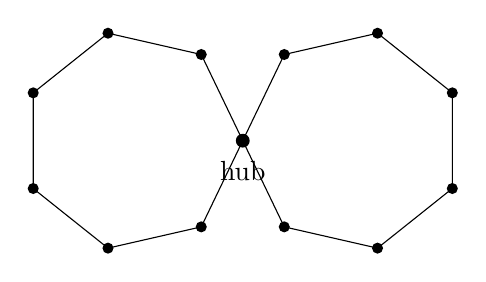
\begin{tikzpicture}[x=0.7cm,y=0.7cm]
\begin{scope}[shift={(-2,0)}]
\coordinate (l0) at (0:2);
\foreach \i in {1,...,6} {\coordinate (l\i) at ({360*\i/7}:2);}
\draw (l0)--(l1)--(l2)--(l3)--(l4)--(l5)--(l6)--cycle;
\foreach \i in {1,...,6} {\fill (l\i) circle (2pt);}
\end{scope}
\begin{scope}[shift={(2,0)}]
\coordinate (r0) at (180:2);
\foreach \i in {1,...,6} {\coordinate (r\i) at ({180+360*\i/7}:2);}
\draw (r0)--(r1)--(r2)--(r3)--(r4)--(r5)--(r6)--cycle;
\foreach \i in {1,...,6} {\fill (r\i) circle (2pt);}
\end{scope}
\fill (0,0) circle (2.5pt) node[below=4pt] {hub};
\end{tikzpicture}
\caption{The support of the order-thirteen seed before the positive completely positive reserve is added. Every proper principal block is completely positive; the full matrix is not.}
\label{fig:bouquet}
\end{figure}

The proof rests on two classical ingredients: a comparison matrix and a bordered Schur complement. We state the exact forms needed, rather than treating the threshold phenomenon as new \cite{Drew,Barioli}.

For a symmetric nonnegative matrix $X$, its \emph{comparison matrix} $M(X)$ keeps the diagonal and negates every off-diagonal entry. Its support graph has an edge $ij$ when $i\ne j$ and $X_{ij}>0$. A graph is triangle-free when no three vertices are pairwise adjacent.

\begin{lemma}[Comparison criterion]\label{lem:comparison}
If $X\ge0$ is symmetric and $M(X)\succeq0$, then $X$ is completely positive. Conversely, if the support graph is triangle-free and $X$ is completely positive, then $M(X)\succeq0$.
\end{lemma}
\begin{proof}
First suppose $M(X)\succ0$. Write $M(X)=tI-K$ with $K\ge0$ and $t>\rho(K)$, taking $t$ sufficiently large. Its inverse is nonnegative by the Neumann series. Thus $d=M(X)^{-1}\mathbf1>0$. The nonnegative matrix $\diag(d)X\diag(d)$ has diagonal excess
\[
 d_i^2X_{ii}-\sum_{j\ne i}X_{ij}d_id_j
 =d_i(M(X)d)_i=d_i>0.
\]
It is therefore the sum of singleton squares with these coefficients and the squares $(e_i+e_j)(e_i+e_j)\T$ with coefficients $X_{ij}d_id_j$. Undoing positive diagonal congruence gives a completely positive factorization of $X$. If $M(X)$ is only semidefinite, apply the result to $X+\eta I$ and let $\eta\downarrow0$, using closedness of $\CP$.

Conversely, in a nonnegative rank-one factorization, a zero entry $X_{ij}=0$ forces every factor to vanish at $i$ or $j$. Each factor is supported on a clique. In a triangle-free graph this support has at most two vertices. Negating the off-diagonal entry of such a rank-one matrix produces another positive semidefinite rank-one matrix. Summing proves $M(X)\succeq0$.
\end{proof}

Let $A_0\in\mathbb S^r(\Q)$ be positive definite and nonnegative, with support a disjoint union of paths and positive edge weights. Singletons are allowed, and components are labeled consecutively. Let $c\in\Q_+^r$ have no two adjacent positive entries. Attaching a hub at these coordinates gives a triangle-free graph $G$. Define
\begin{equation}\label{eq:thresholds}
\begin{gathered}
 M_0=M(A_0),\qquad v=M_0^{-1}c,\qquad
 \alpha=c\T A_0^{-1}c,\qquad \beta=c\T M_0^{-1}c,\\
 F(a)=\begin{pmatrix}A_0&c\\c\T&a\end{pmatrix}.
\end{gathered}
\end{equation}
Changing only the hub diagonal now gives an exact interval. The interval is the constructive route to seeds; its comparison and bordered-matrix antecedents are discussed in \cite{Drew,Barioli}.

\begin{theorem}[Graphical seed interval]\label{thm:seedinterval}
For $a\ge0$,
\[
 F(a)\succ0\quad\Longleftrightarrow\quad a>\alpha,
 \qquad
 F(a)\in\CP_{r+1}\quad\Longleftrightarrow\quad a\ge\beta.
\]
The interval $(\alpha,\beta)$ is nonempty exactly when, in some path component, the hub attaches to both bipartition classes. Under the no-adjacent-attachment assumption, this is equivalent to $G$ containing an odd cycle of length at least five.

For every rational $a$ in this interval, an explicit positive diagonal congruence and completely positive reserve turn $F(a)$ into a certified seed for $T_r$. Hence Theorem~\ref{thm:amplification} applies from $T_{r+1}$ and every bounded region of the same face.
\end{theorem}
\begin{proof}
Give the two classes of each path opposite signs and let $J$ be the resulting diagonal sign matrix. Then $M_0=JA_0J\succ0$. Its inverse is nonnegative, and strictly positive within each connected component: the Neumann series contains a positive walk term between any two connected vertices. The Schur complement of $A_0$ gives the first equivalence. The Schur complement of $M_0$, together with Lemma~\ref{lem:comparison}, gives the second.

If the bipartition is $U\cup V$, sign switching also gives
\begin{equation}\label{eq:thresholdgap}
 \beta-\alpha
 =4\sum_{\substack{i\in U\\j\in V}}c_ic_j(M_0^{-1})_{ij}.
\end{equation}
Terms between different components vanish. The sum is positive precisely when two opposite-colored coordinates are attached in one component. Their path distance is odd; excluding adjacent attachments makes it at least three. Adding the hub produces an odd cycle of length at least five. Conversely, deleting the hub from any cycle leaves the path between its two attachments.

We construct both the separator and the normal reserve. For a triangle-free graph,
\[
 Q_G=\mathbf1\mathbf1\T-2\operatorname{Adj}(G)
\]
is copositive by the Motzkin--Straus bound \cite{MS}. Here is the short argument needed. On the nonnegative simplex, maximize the sum of edge products and choose a maximizer with smallest support. If two positive coordinates are nonadjacent, moving their total mass to the one with larger neighbor sum does not decrease the objective and reduces the support. Thus the support is a clique, of size at most two; its edge product is at most $1/4$. Homogeneity proves copositivity.

Let $W_F=\diag(v,1)Q_G\diag(v,1)$. Using $M_0v=c$ gives the decisive pairing
\begin{equation}\label{eq:graphwitness}
 \ip{W_F}{F(a)}=v\T M_0v-2c\T v+a=a-\beta<0.
\end{equation}
Zero coordinates of $v$ are allowed.

Next set $d=M_0^{-1}\mathbf1>0$ and $D=\diag(d,1)$. The leading block has the exact decomposition
\begin{equation}\label{eq:normalrealization}
 \diag(d)A_0\diag(d)=
 \sum_i d_i e_ie_i\T+
 \sum_{ij\in E(A_0)}(A_0)_{ij}d_id_j(e_i+e_j)(e_i+e_j)\T.
\end{equation}
All displayed vectors minimize $T_r$, since each support edge joins consecutive coordinates. To obtain a spanning positive reserve, let $C_n$ be the sum of all interval squares in order $n=r+1$, as in \eqref{eq:canonicalseed}, and put
\begin{equation}\label{eq:seedassembly}
\begin{gathered}
 W'=D^{-1}W_FD^{-1},\quad \gamma_0=\beta-a,\quad
 w'=1+\sum_{ij}|W'_{ij}|,\quad
 \varepsilon=\frac{\gamma_0}{4w'\tr C_n},\\
 B=DF(a)D+\varepsilon C_n.
\end{gathered}
\end{equation}
This $B$ is rational, positive definite, and strictly positive. Restricting the intervals to the first $r$ coordinates supplies every top interval with positive coefficient.

For completeness,
\begin{equation}\label{eq:Tidentity}
 T_j[x]=\frac12\left(x_1^2+x_j^2+
                 \sum_{i=1}^{j-1}(x_i-x_{i+1})^2\right).
\end{equation}
This is positive for every nonzero real $x$ and is an integer for integer $x$. Its minimum on nonzero nonnegative integer vectors is one, attained at interval indicators. Their squares span: singleton values determine the diagonal, and the four-term difference obtained by deleting either endpoint or both from an interval recovers $2X_{ij}$. Thus $T_r$ is perfect and the reserve meets Definition~\ref{def:seed}. Finally,
$|\ip{W'}{\varepsilon C_n}|\le\varepsilon w'\tr C_n=\gamma_0/4$,
so $\ip{W'}B\le-3\gamma_0/4<0$. The face contains $T_n$ by \eqref{eq:Tidentity}.
\end{proof}

This characterizes the stated graphical class, not arbitrary support graphs. If all attachments lie in one color class per component, \eqref{eq:thresholdgap} vanishes and no hub diagonal gives a positive definite nonmember. Triangle-freeness is also substantive: $J_3$ is completely positive but its comparison matrix $2I-J_3$ is indefinite.

\subsection{All proper principal blocks and a perturbation ball}
To make every proper block pass, choose the hub diagonal just below its full comparison threshold but above every deletion threshold. Let every path component be attached at both endpoints, with any singleton component attached positively. Exclude two-vertex components, which would create triangles, and require at least one component with an even number of vertices $s\ge4$. Then $v=M_0^{-1}c$ is strictly positive and $\beta>\alpha$. Put
\begin{equation}\label{eq:deletionmargins}
 \Delta_i=\frac{v_i^2}{(M_0^{-1})_{ii}}>0,\qquad
 0<\delta<\min\{\beta-\alpha,\min_i\Delta_i\},\qquad
 a=\beta-\delta,
\end{equation}
with all data rational. Half the displayed minimum is one exact choice.

\begin{theorem}[Principal-minimal seeds]\label{thm:minimal}
The matrix $F(a)$ defined above is positive definite, nonnegative, and not completely positive, while every proper principal submatrix is completely positive. The seed $B$ in \eqref{eq:seedassembly} has the same properties and strictly positive entries.

For the interval reserve, choosing $\zeta\le\varepsilon/8$ in \eqref{eq:robustconstants} ensures that every proper principal submatrix of every amplified input in \eqref{eq:ball} is completely positive. Thus no copositive matrix supported on a proper principal index set, nor any nonnegative combination of such matrices, separates these inputs.
\end{theorem}
\begin{proof}
The full Schur complement is $a-\alpha=\beta-\alpha-\delta>0$, but its comparison Schur complement is $a-\beta=-\delta<0$. For deletion of top coordinate $i$, block inversion gives
\begin{equation}\label{eq:deletionidentity}
 \beta-c_{-i}\T(M_0[-i])^{-1}c_{-i}
 =\frac{v_i^2}{(M_0^{-1})_{ii}}=\Delta_i.
\end{equation}
Here $M_0[-i]$ means deletion of row and column $i$. To see the identity directly, partition $M_0$ at $i$; the inverse Schur formula makes the difference the square of the residual component of $c$, divided by the positive scalar Schur complement. Its inverse is $(M_0^{-1})_{ii}$ and its residual divided by that complement is $v_i$, giving the displayed expression.

The comparison matrix of $F(a)[-i]$ has positive Schur complement $\Delta_i-\delta$. It is positive definite and hence $F(a)[-i]$ is completely positive by Lemma~\ref{lem:comparison}. Deleting the hub leaves $A_0$, with positive definite comparison matrix, so that block is also completely positive. Every smaller principal submatrix is contained in a one-coordinate deletion. Positive diagonal congruence and addition of a completely positive matrix preserve all these conclusions. The separator estimate in \eqref{eq:seedassembly} preserves full nonmembership.

We give a uniform radius, including all proper index sets. Regard the interval squares as a basis of $\mathbb S^n$ in upper-triangular coordinates. The inverse coefficient map consists of four-term differences and has maximum absolute row sum at most four. A perturbation $Z$ with $\norm Z_F\le\varepsilon/8$ therefore changes each coefficient of $\varepsilon C_n$ by at most $\varepsilon/2$. All coefficients remain positive, so $\varepsilon C_n+Z$ is completely positive.

For any proper principal set $I$, embed a perturbation of its block by zeros outside $I$, apply the preceding fact, and restrict back to $I$. Adding the already completely positive unreserved principal block proves stability for every $I$ at once. For an amplified perturbation, undo the normalization and the diagonal scaling. Since every diagonal entry of $D_N$ is at least one, its inverse does not increase the Frobenius norm. Thus $\zeta\le\varepsilon/8$ suffices throughout \eqref{eq:ball}.

Finally, complete positivity of $A[I]$ gives $\ip{A[I]}{Q[I]}\ge0$ for every copositive candidate supported on $I$. Summing proves the assertion for nonnegative combinations.
\end{proof}

The order-thirteen numbers can be recovered by a short determinant recurrence. Write $d_k=\det(I_k-\operatorname{Adj}(P_k)/4)$. Then $d_0=d_1=1$ and $d_k=d_{k-1}-d_{k-2}/16$. For $i\le j$, its inverse has entry
\[
 (M_0^{-1})_{ij}=4^{i-j}\frac{d_{i-1}d_{6-j}}{d_6}
\]
on each six-vertex block, with $d_5=195/256$ and $d_6=2911/4096$. Sign switching gives the inverse of $K_6$. Hence one path contributes
\[
 \alpha_0=\frac{152}{71},\qquad \beta_0=\frac{88}{41},\qquad
 \beta_0-\alpha_0=\frac{16}{2911}.
\]
In the two-component matrix, $\min_i\Delta_i=71/8610$. Taking
$\delta=71/17220$ gives exactly $a=73849/17220$ and satisfies \eqref{eq:deletionmargins}. This proves all the claims made above for that example. In particular each seven-cycle principal block passes the completely positive test, while the full matrix fails. Repeating six-vertex components gives examples of unbounded order.

Single even-order paths give another family. With $s\in2\Z$, $s\ge4$, take $A_0=I_s+\operatorname{Adj}(P_s)/4$ and $c=e_1+e_s$. The support is a chordless odd cycle of length $s+1$. Such support obstructions are classical \cite{Kogan}; here they provide qualifying seeds for amplification. Lengths seven and nine have no five-cycle principal support. Weighted nonadjacent attachments and several path components are also covered by Theorem~\ref{thm:seedinterval}; changing the seed's graphical support is separate from the later diagonal amplification.

\subsection{Branched perfect blocks and bounded starting regions}
The leading normal geometry need not be tridiagonal. Let $T$ be a tree with
$H_T=I_r-\operatorname{Adj}(T)/2\succ0$. For every unordered pair, including a repeated pair, let $p_{ij}$ be the indicator of the unique tree path. Then $H_T[p_{ij}]=1$. These are a spanning collection of minimal vectors, not necessarily the complete list. Their squares span $\mathbb S^r$: deleting either endpoint or both from a path gives a four-term difference equal to $2X_{ij}$, and repeated pairs give the diagonal. Since $H_T[x]$ is positive and integral on nonzero integer vectors, $H_T$ is a positive definite perfect vertex.

The same construction works whenever the leading support is a forest contained in $T$. The hypotheses that the hub attachments are nonadjacent and the resulting graph is triangle-free remain in force. The comparison and Schur arguments are unchanged, and the singleton and support-edge vectors in \eqref{eq:normalrealization} are minimal for $H_T$. Use the reserve
\begin{equation}\label{eq:treereserve}
 \mathcal B_T=\sum_{i\le j}\left[
 (p_{ij},0)(p_{ij},0)\T+(p_{ij},1)(p_{ij},1)\T\right]+e_ne_n\T.
\end{equation}
Its leading block is twice the sum of the path squares and all its entries are positive. Its atoms span $\mathbb S^n$: the unlifted paths span the leading block, the final singleton gives the last entry, and lifted singleton paths give the cross entries. Adding $\varepsilon\mathcal B_T$ with $\varepsilon=(\beta-a)/(4w'\tr\mathcal B_T)$ proves the seed conditions exactly as before.

If all proper principal blocks passed before this addition, they still pass and become interior completely positive points. A finite radius is obtained by selecting an atom basis with coefficients at least one in \eqref{eq:treereserve}. If $U$ is its coordinate matrix and $L_U=\norm{U^{-1}}_\infty$, then
$\norm Z_F\le\varepsilon/(2\max(1,L_U))$ preserves positivity of the basis coefficients. The proof of Theorem~\ref{thm:minimal} then gives the principal-block barrier throughout the corresponding amplified ball.

For the branched $D_r$ tree, $r\ge4$, use edges $i(i+1)$ for $1\le i\le r-2$ and $(r-2)r$. The matrix $H_T$ is half the Gram matrix of
$e_1-e_2,\ldots,e_{r-1}-e_r,e_{r-1}+e_r$, so it is positive definite. Adding the new vertex at old vertex $1$ gives a $D_{r+1}$ perfect form with leading block $H_T$, hence an explicit start. On $D_7$, the seed $A_0=I+\operatorname{Adj}(D_7)/4$ with hub attachments at $1$ and $6$ has a seven-cycle and a pendant branch. Choosing its diagonal by \eqref{eq:deletionmargins} gives an order-eight principal-minimal seed. This changes both the seed support and the leading perfect block.

In the canonical face, additional explicit starts are
$P_a=S_a^{-\mathsf T}T_nS_a^{-1}$ for fixed $a\in\Z_+^r$. Indeed $S_a^{-1}(u,y)=(u-ay,y)$ is a nonzero integer vector, and $T_n$ has minimum one on the full integer lattice by \eqref{eq:Tidentity}. Thus $P_a$ is feasible. The forward images $S_a(v,y)=(v+ay,y)$ of the interval minimizers are nonnegative and their squares still span, proving perfectness. Every fixed bounded collection of these starts, and all vertices in any fixed bounded cross-column region of the same face, is covered simultaneously.

\subsection{Further sparsity-limited tests}
A symmetric matrix is called \emph{SPN} if it is a sum of a positive semidefinite matrix and an entrywise nonnegative matrix. A graph is SPN if every copositive matrix with off-diagonal support contained in that graph is SPN. Any copositive candidate confined to such a support has nonnegative pairing with a doubly nonnegative input, regardless of how the candidate is found.

For example, partition the leaf coordinates into groups of at most three. Allow every entry within each group, all hub spokes, and all diagonals. This support is a union of cliques of order at most four meeting only at the hub, and is SPN \cite[Corollaries~4.4 and~5.3]{SPN}. It permits small full-block corrections beyond the diagonal correction in Corollary~\ref{cor:stored}. The forest and small-block results used here are classical and unaffected by the corrigendum \cite{SPNcorr}; no general triangular-book assertion is used.

The new algorithmic consequence of Lemma~\ref{lem:arrow} is simultaneous failure for every stored direction, because confinement puts them all in the arrow space. The principal-minimal seeds supply a different barrier: all proper principal tests fail on the whole certified ball. Neither assertion covers arbitrary off-diagonal corrections or combinations with unrelated non-arrow matrices.

\section{Consequences and limits}\label{sec:scope}
The results separate the size of a copositive certificate from the number of adjacent pivots needed to reach one. A finite positive reserve turns each certified seed into robust lower bounds for every improving choice from a bounded region of one fixed-block face; the common separator remains short. Independently, the fixed-block epigraph has finite local configurations and intrinsic graph growth of exact degree equal to the block order. Graphically different seeds, including branched leading blocks and principal-minimal nonmembers, show how the amplification extends beyond the five-cycle. The excluded methods are precise: unrelated global certificates, distant input-dependent restarts, nonadjacent jumps, and non-descending steps. Bounded-region starts with different leading perfect blocks are also outside the theorem; the same strict normal reserve cannot favor two distinct perfect vertices. Intrinsic graph distance does not control shortcuts outside the face. None of these results decides eventual termination under a suitable pivot rule or gives a general polynomial-time recognition algorithm. Exact-arithmetic programs and certificate data accompany the paper as supplementary material.

\appendix
\section{Explicit canonical constants}\label{app:canonical}
This appendix gives a fully numerical specialization of the seed theorem. It also shows that the same confinement argument applies at larger scales, with the stated normalization and separator margins.

Use $B,W_0,\epsilon$ from Section~\ref{sec:canonicalseed}. Write
$B=\begin{pmatrix}B_0&c_0\\c_0\T&a_0\end{pmatrix}$ and put
\begin{equation}\label{eq:canonicalparameters}
\begin{gathered}
 r=n-1,\quad d=n(n+1)/2,\quad q=2n,\quad Y=2q^r,\\
 U=2Yn^2(t+1),\qquad
 E=(d-1)!(2U^2)^{d-1},\qquad N=20000n^3E^2.
\end{gathered}
\end{equation}
The matrices in Corollary~\ref{cor:canonical} are
\begin{equation}\label{eq:canonicalcenters}
 S_N=\diag(NI_r,1),\qquad
 A_{n,t}=\frac{S_NBS_N}{4nN^2},\qquad
 W_{n,t}=S_N^{-1}W_0S_N^{-1}+\frac{I_n}{20nN^2}.
\end{equation}

\subsection{Seed and separator reserves}
The seed has
\begin{equation}\label{eq:canonicalreserves}
 B\succ I_n/40,\quad B_{ij}\ge\epsilon,\quad
 \norm B_F\le3n,\quad
 0<a_0<2,\quad c_0>0,\quad \norm{c_0}_1<2.
\end{equation}
Indeed all diagonal entries of $D$ are at least one, and the least eigenvalue of $F$ is greater than $1/40$. The interval representation of $C_n$ makes it positive definite with positive entries. Its trace is $n(n+1)(n+2)/6\le n^3$, so $\norm{C_n}_F\le n^3$. Every seed diagonal and off-diagonal entry is less than three, which gives the Frobenius estimate. Finally,
\[
 a_0=1+\epsilon n,\qquad
 (c_0)_i=\tfrac35(\mathbf1_{i=1}+\mathbf1_{i=4})+\epsilon i,
\]
proving the last assertions.

The leading block of $DFD$ is a sum of the interval squares with nonzero weights
\[
\begin{array}{c|rrrrrrr}
 \text{interval}&[1]&[2]&[3]&[4]&[1,2]&[2,3]&[3,4]\\ \hline
 \text{weight}&1/25&8/125&8/125&1/25&24/25&192/125&24/25
\end{array}
\]
and singleton weight one at every further top coordinate. These weights give off-diagonal entries $24/25,192/125,24/25$ and diagonal entries $1,64/25,64/25,1$. Adding $\epsilon C_n$ gives every top interval a coefficient at least $\epsilon$. Its squares span by \eqref{eq:Tidentity} and the four-term interval identity. Moreover their unreserved weights sum to $r-42/125>1$, so
\[
 \ip{B_0}{T_r}\ge1.
\]
The seed entries have common denominator $500n^3$: the unreserved part has denominator dividing $125$, and the reserve denominator divides $100n^3$.

The Horn witness has $\norm{W_0}_F\le5$, since inverse diagonal congruence contracts its entries. Its pairing with $DFD$ is $5-6=-1$. Hence
\[
 \ip{W_0}B\le-1+5\epsilon\norm{C_n}_F\le-\frac{19}{20}.
\]
This proves all seed requirements analytically.

The identity addition in \eqref{eq:canonicalcenters} changes its unnormalized pairing by at most $3/20$, since $\tr(S_NBS_N)\le3nN^2$. Thus
\begin{equation}\label{eq:canonicalpairing}
 \ip{W_{n,t}}{S_NBS_N}\le-\frac45,\qquad
 \ip{W_{n,t}}{A_{n,t}}\le-\frac1{5nN^2},
 \qquad \norm{W_{n,t}}_F\le6.
\end{equation}
Copositivity of the first summand gives the strict margin in \eqref{eq:canonicalmargins}. The center satisfies
\[
 \norm{A_{n,t}}_F\le\frac34,\qquad
 \lambda_{\min}(A_{n,t})>\frac1{160nN^2},\qquad
 (A_{n,t})_{ij}\ge\frac1{400n^4N^2}.
\]
A Frobenius perturbation of radius $\rho=1/(1600n^4N^2)$ preserves positive definiteness, strict entrywise positivity, and norm at most one. It increases the witness pairing by at most $6\rho$, leaving the bound $-1/(6nN^2)$. Division by the witness norm gives distance at least $1/(36nN^2)$. This proves all numerical claims in the corollary.

\subsection{The confinement scale}
We check that \eqref{eq:canonicalparameters} is large enough for every improving choice. In the height and domination constants, take $H=T_r$, $b_0=1/2$, and $\zeta_{\mathrm{can}}=\epsilon/4$. This last choice is the bound on the perturbation after rescaling by $4nN^2$. Only $\zeta_{\mathrm{can}}\le\min B_{ij}/2$ is needed for the objective argument; nonmembership and robustness have just been proved.

Use $q,Y$ in \eqref{eq:canonicalparameters}, choose $t_H=n$, and write
$K=Y+n$ and $E_*=(d-1)!(2K^2)^{d-1}$. The inverse formula
\[
 (T_r^{-1})_{ij}=\frac{2\min(i,j)(n-\max(i,j))}{n}
\]
gives $h\le2$ and $j\le n^2/4$. The constants \eqref{eq:heightconstants} then satisfy
\[
 B_*\le13/2,\quad Z_*\le2n^2,\quad T_*\le2n^3,\quad
 P_*\le9n^5,\quad\alpha\ge1.
\]
Together with $D_C=500n^3$ and \eqref{eq:canonicalreserves}, these imply
\[
 u\le8n^3E_*,\quad v\le9n^6E_*,\quad
 u_2\le26,\quad v_2\le9n^2/400.
\]
Consequently the threshold in \eqref{eq:Gamma} for the domination inequalities is at most $30000n^9E_*$. Put $M=t+1$. Since $Y\ge n$,
\[
 \frac UK\ge n^2M,\qquad
 \frac E{E_*}\ge(n^2M)^{2(d-1)}
                   \ge n^4M^2\ge2n^3M.
\]
It follows that
\[
 \frac NM=\frac{20000n^3E^2}{M}
       \ge80000n^9ME_*^2\ge30000n^9E_*.
\]
Thus Lemma~\ref{lem:confinement} applies to the rescaled objective
$4nN^2A=S_NBS_N+Z$, with $\norm Z_F\le\epsilon/4$.
Its vertex gap, finite endpoints, and the arrow barrier give the induction exactly as in Theorem~\ref{thm:amplification}. This proves the pivot assertion of Corollary~\ref{cor:canonical} with all of its allowed tests.

For fixed $n$, the scale is a constant times $(t+1)^{4(d-1)}$, so the center and witness have $O_n(\log(t+1))$ binary length. Conversely,
$(A_{n,t})_{nn}=(1+\epsilon n)/(4nN^2)$ has a fixed nonzero rational numerator before reduction. Its denominator supplies the matching lower bound. The reciprocal-distance term is bounded by \eqref{eq:canonicalmargins}, completing the encoding claim.

\section*{Declaration of generative AI and AI-assisted technologies in the manuscript preparation process}
OpenAI Codex was used for manuscript drafting, literature checks, and LaTeX editing. It also assisted with exact-arithmetic verification of explicit instances and preparation of the computational supplement. The author retains full responsibility for the content.
\begin{thebibliography}{20}\raggedright
\bibitem{Barioli} F. Barioli, Decreasing diagonal elements in completely positive matrices, \emph{Rendiconti del Seminario Matematico della Universit\`a di Padova} \textbf{100} (1998), 13--25. \url{https://www.numdam.org/item/RSMUP_1998__100__13_0/}.
\bibitem{DS} V. Dannenberg and A. Sch\"urmann, Perfect copositive matrices, \emph{Communications in Mathematics} \textbf{31} (2023), no.~2, 137--156. \href{https://doi.org/10.46298/cm.11141}{doi:10.46298/cm.11141}.
\bibitem{Diananda} P. H. Diananda, On non-negative forms in real variables some or all of which are non-negative, \emph{Proceedings of the Cambridge Philosophical Society} \textbf{58} (1962), 17--25. \href{https://doi.org/10.1017/S0305004100036185}{doi:10.1017/S0305004100036185}.
\bibitem{Drew} J. H. Drew, C. R. Johnson, and R. Loewy, Completely positive matrices associated with M-matrices, \emph{Linear and Multilinear Algebra} \textbf{37} (1994), 303--310. \href{https://doi.org/10.1080/03081089408818334}{doi:10.1080/03081089408818334}.
\bibitem{DSV} M. Dutour Sikiri\'c, A. Sch\"urmann, and F. Vallentin, A simplex algorithm for rational cp-factorization, \emph{Mathematical Programming} \textbf{187} (2021), 25--45. \href{https://doi.org/10.1007/s10107-020-01467-4}{doi:10.1007/s10107-020-01467-4}.
\bibitem{Inhom} M. Dutour Sikiri\'c, A. Sch\"urmann, and F. Vallentin, Inhomogeneous extreme forms, \emph{Annales de l'Institut Fourier} \textbf{62} (2012), 2227--2255. \href{https://doi.org/10.5802/aif.2748}{doi:10.5802/aif.2748}.
\bibitem{HN} M. Hall, Jr. and M. Newman, Copositive and completely positive quadratic forms, \emph{Proceedings of the Cambridge Philosophical Society} \textbf{59} (1963), 329--339. \href{https://doi.org/10.1017/S0305004100036951}{doi:10.1017/S0305004100036951}.
\bibitem{Kogan} N. Kogan and A. Berman, Characterization of completely positive graphs, \emph{Discrete Mathematics} \textbf{114} (1993), 297--304. \href{https://doi.org/10.1016/0012-365X(93)90374-3}{doi:10.1016/0012-365X(93)90374-3}.
\bibitem{MM} J. E. Maxfield and H. Minc, On the matrix equation $X'X=A$, \emph{Proceedings of the Edinburgh Mathematical Society} \textbf{13} (1962), 125--129. \href{https://doi.org/10.1017/S0013091500014681}{doi:10.1017/S0013091500014681}.
\bibitem{MS} T. S. Motzkin and E. G. Straus, Maxima for graphs and a new proof of a theorem of Tur\'an, \emph{Canadian Journal of Mathematics} \textbf{17} (1965), 533--540. \href{https://doi.org/10.4153/CJM-1965-053-6}{doi:10.4153/CJM-1965-053-6}.
\bibitem{OS} A. Oertel and A. Sch\"urmann, Generalized perfect matrices, preprint, arXiv:2602.05841v2 (2026). \url{https://arxiv.org/abs/2602.05841v2}.
\bibitem{SPN} N. Shaked-Monderer, SPN graphs: When copositive = SPN, \emph{Linear Algebra and its Applications} \textbf{509} (2016), 82--113. \href{https://doi.org/10.1016/j.laa.2016.07.018}{doi:10.1016/j.laa.2016.07.018}.
\bibitem{SPNcorr} N. Shaked-Monderer, Corrigendum to SPN graphs: When copositive = SPN, \emph{Linear Algebra and its Applications} \textbf{541} (2018), 285--286. \url{https://arxiv.org/abs/1712.05115}.
\bibitem{SZ} T. \v Strekelj and A. Zalar, Construction of exceptional copositive matrices, \emph{Linear Algebra and its Applications} \textbf{727} (2025), 368--384. \href{https://doi.org/10.1016/j.laa.2025.08.010}{doi:10.1016/j.laa.2025.08.010}.
\end{thebibliography}

\end{document}
